% Do not forget to include Introduction
%---------------------------------------------------------------
\chapter{Introduction}
% uncomment the following line to create an unnumbered chapter
%\chapter*{Introduction}\addcontentsline{toc}{chapter}{Introduction}\markboth{Introduction}{Introduction}
%---------------------------------------------------------------
\setcounter{page}{1}

% TODO: prozkoumat? https://en.wikipedia.org/wiki/Natural_deduction#Gentzen-style_propositional_logic
% TODO: prozkoumat? https://en.wikipedia.org/wiki/Natural_deduction#Substitution_theorem

\section{SAT}
\subsection{SAT formulace}
\subsection{SAT řešiče}
\subsubsection{DPLL}
\subsubsection{CDCL}


\section{SMT}

Satisfiability Modulo Theories (SMT) je rozšíření SAT, které se zabývá rozhodováním o tom,
zda existuje přiřazení proměnných, které splňuje danou logickou formuli.
SMT se používá v různých oblastech, jako je verifikace softwaru, analýza programů a automatizované dokazování.



\subsection{Standard SMT-LIB}
\subsection{SMT řešiče}
\subsubsection{Eager přístup}
\subsubsection{Lazy přístup}
\subsubsection{Alt-Ergo}
\subsubsection{CVC}
\subsubsection{Z3}


\chapter{Hoareova logika}

Formální systém označovaný jako Hoareova logika byl navržen a popsán
britským matematikem a informatikem C. A. R. Hoarem v roce 1969. \cite{Hoare1969}
Jedná se o formální systém pro popis a analýzu počítačových programů,
který pro důkaz správnosti programů používá předpoklady (preconditions) a následky (postconditions).

Program popisujeme pomocí Hoareovy trojice

\begin{equation*}
    \{P\} \  Q \  \{R\}
\end{equation*}

kde $P$ jsou předpoklady popisující stav systému před provedením programu,
$Q$ je daný program (příkaz či sekvence příkazů)
a $R$ jsou následky, které popisují stav systému po provedení tohoto programu.
Takto popsaný systém čteme následovně:
``Při splněných předpokladech $P$ budou po provedení programu $Q$ zaručeny následky $R$``.

Hoare v roce 1969 definoval trojici jako $P \ \{ Q \} \  R$,
ale v současnosti se častěji setkáme se zápisem $\{ P \} \  Q \ \{ R \}$.

Předpoklady a následky jsou vyjádřeny jako logické formule,
které popisují vlastnosti proměnných programu v určitém okamžiku.
Následující příklad reprezentuje program, který předpokládá na vstupu nezápornou hodnotu v proměnné $x$
a po provedení programu $Q$ bude zajištěno, že hodnota proměnné $x$ bude kladná (ostře větší než 0).

\begin{equation*}
    \{ x \geq 0 \} \  x \coloneqq x + 1 \  \{ x > 0 \}
\end{equation*}

Předpoklad může být také prázdný, což znamená, že program nevyžaduje žádné předpoklady
a formálně to lze zapsat jako $\{ true \} \  Q \  \{ R \}$.
Pokud je předpoklad prázdný, předpokládáme, že program může být spuštěn
v libovolném stavu systému nebo s libovolnými hodnotami proměnných.
Takový program může vypadat následovně:

\begin{equation*}
    \{ true \} \  x \coloneqq 10 \  \{ x > 0 \}
\end{equation*}

% TODO: zminit, ze toto je validni program, ale casto nam tento vysledek nic nerika a je potreba
% TODO: jeste pridat podminky na hodnoty promennych v ruznem case atd...

\section{Axiom přiřazení}

Axiom přiřazení je základním pravidlem Hoareovy logiky a nedílnou součástí každého počítačového programu.
Přiřazení je operace obecně zapsaná ve tvaru

\begin{equation*}
    x \coloneqq f
\end{equation*}

kde $x$ je proměnná a $f$ je výraz bez vedlejších efektů (side effect),
který ale může obsahovat proměnnou $x$, např. $x \coloneqq x + 1$.

Chceme zajistit, že jakékoli tvrzení $T$ platné o $f$
je také platné o hodnotě proměnné $x$ po provedení přiřazení.
Označíme si $T[x \rightarrow f]$ tvrzení $T$ ve kterém výskyt proměnné $x$ nahradíme výrazem $f$ (substituce).

Poté můžeme definovat axiom přiřazení jako

\begin{equation*}
    \{ T[x \rightarrow f] \} \  x \coloneqq f \  \{ T \}
\end{equation*}

Tento zápis říká, že pokud je pravdivé tvrzení $T$, ve kterém
je výskyt proměnné $x$ nahrazen výrazem $f$, pak po provedení přiřazení
je tvrzení $T$ pravdivé také pro proměnnou $x$.
Jedná se tedy o šablonu (schéma) axiomu,
kterou lze použít pro libovolné tvrzení $T$, proměnnou $x$ a výraz $f$.

% TODO: The assignment axiom proposed by Hoare does not apply when more than one name may refer to the same stored value. For example,
% TODO: end of https://en.wikipedia.org/wiki/Hoare_logic#Assignment_axiom_schema
% TODO: toto ma mozna konsekvence do Frama-C pri volne pametoveho modelu a proc
% TODO: nektere tvrzeni neprojdou na pointerech a rekurzivnich strukturach

\section{Pravidlo důsledku}

Pravidlo důsledku (rule of consequence) je metoda umožnující
tvorbu nových logických tvrzení z již existujících a dokázaných tvrzení.
Základní aplikací této metody je pravidlo \textbf{rozšíření předpokladu}
a pravidlo \textbf{zůžení následku}.
Předpokládejme platnosti $\{ P \} \  Q \  \{ R \}$.

Máme-li rozšířený předpoklad $P'$, pro který platí

\begin{equation*}
    P' \implies P
\end{equation*}

můžeme říci, že

\begin{equation*}
    \{ P' \} \  Q \  \{ R \}
\end{equation*}

je také platné tvrzení.

Máme-li zúžený následek $R'$ následku $R$, pro který platí

\begin{equation*}
    R \implies R'
\end{equation*}

můžeme říci, že $\{ P \} \  Q \  \{ R' \}$ je také platné tvrzení.

\section{Pravidlo skládání}

Pravidlo skládání (rule of composition) je pravidlo, které umožňuje
skládat více příkazů do jednoho složeného příkazu a používat je v Hoareově logice.

Máme-li dva příkazy $Q_1$ a $Q_2$, které splňují následující tvrzení

\begin{equation*}
    \{ P_1 \} \  Q_1 \  \{ R_1 \}
\end{equation*}

a

\begin{equation*}
    \{ R_1 \} \  Q_2 \  \{ R_2 \}
\end{equation*}

můžeme říci, že složený příkaz $Q_1; Q_2$ splňuje následující tvrzení

\begin{equation*}
    \{ P_1 \} \  Q_1; Q_2 \  \{ R_2 \}
\end{equation*}

kde $;$ je operátor sekvence příkazů, který říká, že příkaz $Q_1$ bude proveden před příkazem $Q_2$.

Toto pravidlo umožňuje vytvářet složené příkazy z jednodušších příkazů.
Zároveň je možné rozmyslet, že na sekvenci příkazů $Q_1, Q_2, \cdots, Q_n$
lze aplikovat stejné pravidlo skládání, které jsme použili pro dva příkazy
pomocí asociativity operátoru $;$ a závorek. A tedy platí, že

\begin{equation*}
    \{ P \} \  Q_1; Q_2; \  \cdots ; Q_n \  \{ R \}
\end{equation*}

je ekvivalentní s

\begin{equation*}
    \{ P \} \  (Q_1; (Q_2; \  \cdots (Q_{n-1}; Q_n))) \  \{ R \}
\end{equation*}

\section{Pravidlo iterace}

Základním stavebním blokem počítačového programu je cyklus.
V Hoareově logice je cyklus reprezentován pomocí pravidla iterace (rule of iteration)
a využívá $while$ cyklus, který je v programovacích jazycích běžně dostupný a je definován následovně:

\begin{equation*}
    while \  B \  do \  Q
\end{equation*}

kde $Q$ je tělo cyklu, které se v každé iteraci provádí, dokud je podmínka $B$ pravdivá.

Dále definujeme invariant cyklu $I$, který nám pomůže
při rozhodování o správnost cyklu a bude popisovat následky provedení cyklu.
Invariant cyklu je logické tvrzení, které musí být pravdivé před vstupem do cyklu,
po ukončení každé iterace cyklu a také po ukončení cyklu.

Formálně můžeme zapsat podmínky pro invariant cyklu $I$ jako

\begin{equation*}
    I \land (\{ B \} \  Q \  \{ I \})
\end{equation*}

První část konjunkce popisuje, že invariant cyklu musí být pravdivý před vstupem do cyklu.
Druhá část konjunkce popisuje, že invariant cyklu musí být pravdivý po provedení těla cyklu $Q$,
pokud se cyklus spustil (podmínka $B$ byla pravdivá).

\begin{remark}
    Invariant cyklu je nezávislý na počtu provedených iterací.
\end{remark}

Pokud cyklus neprovedl žádnou iteraci a zároveň máme zaručeno,
že invariant cyklu $I$ byl pravdivý před vstupem do cyklu,
triviálně platí, že invariant cyklu $I$ je pravdivý i po ukončení cyklu.
Zároveň platí, že cyklus se neprovedl, protože podmínka $B$ byl nepravdivá,

Pokud cyklus provedl alespoň jednu iteraci a zároveň máme zaručeno,
že invariant cyklu $I$ je pravdivý po ukončení těla cyklu $Q$,
znamená to, že invariant cyklu $I$ je pravdivý i po ukončení poslední iterace cyklu.
Zároven platí, že podmínka $B$ je po ukončení cyklu nepravdivá, jinak by cyklus pokračoval v provádění další iterace.

Formálně lze tedy konstrukci $while$ cyklu pomocí Hoareovy logiky zapsat jako

\begin{equation*}
    I \land \{ B \} \  Q \  \{ I \} \implies \{ I \} \  while \  B \  do \  Q \  \{ \neg B \land I \}
\end{equation*}

\chapter{Frama-C}
\subsection{ACSL (ANSI/ISO C Specification Language)}
\subsection{WP (Weakest Precondition)}
\subsection{Paměťové modely}


\chapter{Stainless}
% --genc does not support recursive data types = src/stainless/LinkedList.scala:41:12: Cons and other recursive types are not supported


% The following environment can be used as a mini-introduction for a chapter. Use that any way it pleases you (or comment it out). It can contain, for instance, a summary of the chapter. Or, there can be a quotation.
\begin{chapterabstract}
	\lipsum[1]
\end{chapterabstract}

\lipsum[2][1-4]{} [1]

\lipsum[4]

%---------------------------------------------------------------
\section{Ut enim ad minim veniam}
%---------------------------------------------------------------

\lipsum[6-8]

\begin{figure}
\centering
%\includegraphics[scale=0.4]{pic/index}
\resizebox{\textwidth}{!}{
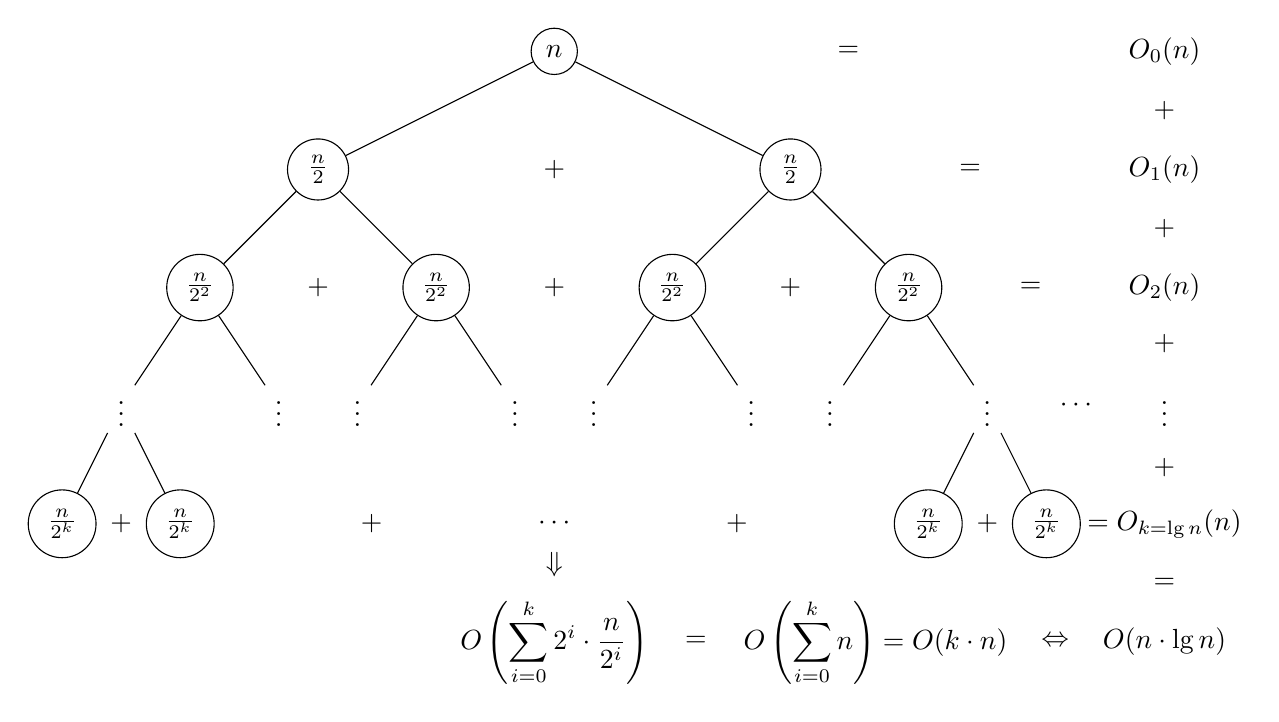
\begin{tikzpicture}[level/.style={sibling distance=60mm/#1}]
\node [circle,draw] (z){$n$}
  child {node [circle,draw] (a) {$\frac{n}{2}$}
    child {node [circle,draw] (b) {$\frac{n}{2^2}$}
      child {node {$\vdots$}
        child {node [circle,draw] (d) {$\frac{n}{2^k}$}}
        child {node [circle,draw] (e) {$\frac{n}{2^k}$}}
      } 
      child {node {$\vdots$}}
    }
    child {node [circle,draw] (g) {$\frac{n}{2^2}$}
      child {node {$\vdots$}}
      child {node {$\vdots$}}
    }
  }
  child {node [circle,draw] (j) {$\frac{n}{2}$}
    child {node [circle,draw] (k) {$\frac{n}{2^2}$}
      child {node {$\vdots$}}
      child {node {$\vdots$}}
    }
  child {node [circle,draw] (l) {$\frac{n}{2^2}$}
    child {node {$\vdots$}}
    child {node (c){$\vdots$}
      child {node [circle,draw] (o) {$\frac{n}{2^k}$}}
      child {node [circle,draw] (p) {$\frac{n}{2^k}$}
          child [grow=right] {node (q) {$ = O_{k = \lg n}(n)$} edge from parent[draw=none]
            child [grow=up] {node (r) {$\vdots$} edge from parent[draw=none]
              child [grow=up] {node (s) {$O_2(n)$} edge from parent[draw=none]
                child [grow=up] {node (t) {$O_1(n)$} edge from parent[draw=none]
                  child [grow=up] {node (u) {$O_0(n)$} edge from parent[draw=none]}
                }
              }
            }
            child [grow=down] {node (v) {$O(n \cdot \lg n)$}edge from parent[draw=none]}
        }
      }
    }
  }
};
\path (a) -- (j) node [midway] {+};
\path (b) -- (g) node [midway] {+};
\path (k) -- (l) node [midway] {+};
\path (k) -- (g) node [midway] {+};
\path (d) -- (e) node [midway] {+};
\path (o) -- (p) node [midway] {+};
\path (o) -- (e) node (x) [midway] {$\cdots$}
  child [grow=down] {
    node (y) {$O\left(\displaystyle\sum_{i = 0}^k 2^i \cdot \frac{n}{2^i}\right)$}
    edge from parent[draw=none]
  };
\path (q) -- (r) node [midway] {+};
\path (s) -- (r) node [midway] {+};
\path (s) -- (t) node [midway] {+};
\path (s) -- (l) node [midway] {=};
\path (t) -- (u) node [midway] {+};
\path (z) -- (u) node [midway] {=};
\path (j) -- (t) node [midway] {=};
\path (y) -- (x) node [midway] {$\Downarrow$};
\path (v) -- (y)
  node (w) [midway] {$O\left(\displaystyle\sum_{i = 0}^k n\right) = O(k \cdot n)$};
\path (q) -- (v) node [midway] {=};
\path (e) -- (x) node [midway] {+};
\path (o) -- (x) node [midway] {+};
\path (y) -- (w) node [midway] {$=$};
\path (v) -- (w) node [midway] {$\Leftrightarrow$};
\path (r) -- (c) node [midway] {$\cdots$};
\end{tikzpicture}}
\caption{Lorem ipsum dolor sit amet}\label{img:index}
\end{figure}

%---------------------------------------------------------------
\section{Ut enim ad minim veniam}
%---------------------------------------------------------------

\lipsum[2-4]

%---------------------------------------------------------------
\subsection{Ut enim ad minim veniam}
%---------------------------------------------------------------

Curabitur ligula sapien, pulvinar a vestibulum quis, facilisis vel sapien. Duis condimentum augue id magna semper rutrum. Aliquam ornare wisi eu metus. Fusce aliquam vestibulum ipsum. Vivamus ac leo pretium faucibus\ref{img:index}.

\begin{itemize}
    \item Ut enim ad minim veniam, quis nostrud
    \item Ut enim ad minim 
    \item Ut enim ad minim veniam, quis 
    \begin{itemize}
        \item Ut enim ad
        \item Ut enim ad
        \begin{itemize}
            \item Ut enim 
            \item Ut enim 
            \begin{itemize}
            \item Ut enim 
            \item Ut enim 
        \end{itemize}
        \end{itemize}
    \end{itemize}
\end{itemize}

\section{Class aptent taciti}


Even though dark mode can be very nice for websites and apps, it does not look good when printed. Consider using white mode when print-screening dark-moded content. The contrast with the white page is too big, as seen in Figure~\ref{fig:Darkmode}.

\begin{figure}[!htbp]
    \centering
    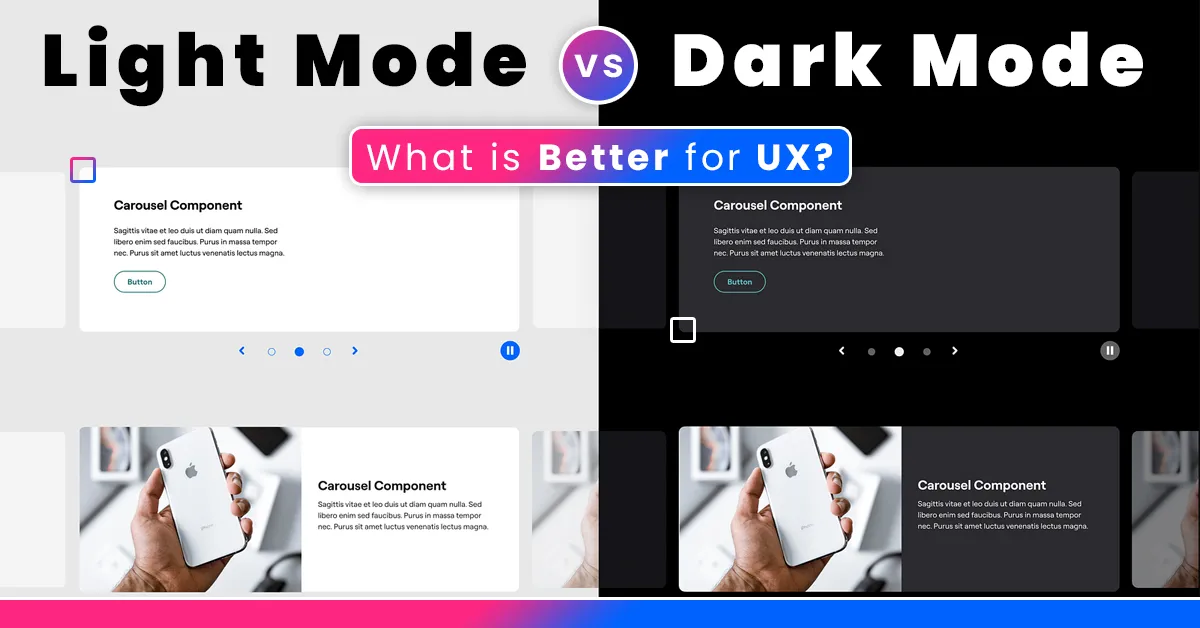
\includegraphics[width=\linewidth]{images/darkmode}
    \caption{White and dark mode comparison.~\cite{darkMode}}
    \label{fig:Darkmode}
\end{figure}


\subsection{Class aptent taciti}

\lipsum[6-7]

\begin{enumerate}
    \item Ut enim ad minim veniam, quis nostrud
    \item Ut enim ad minim 
    \item Ut enim ad minim veniam, quis 
    \begin{enumerate}
        \item Ut enim ad
        \item Ut enim ad
        \begin{enumerate}
            \item Ut enim 
            \item Ut enim 
            \begin{enumerate}
            \item Ut enim 
            \item Ut enim 
        \end{enumerate}
        \end{enumerate}
    \end{enumerate}
\end{enumerate}


%---------------------------------------------------------------
\section{Ut enim ad minim veniam, quis nostrud}
%---------------------------------------------------------------

Ut enim ad minim veniam, quis nostrud exercitation ullamco laboris nisi ut aliquip ex ea commodo consequat. Nulla non arcu lacinia neque faucibus fringilla. Vestibulum erat nulla, ullamcorper nec, rutrum non, nonummy ac, erat. Aliquam erat volutpat. Proin pede metus, vulputate nec, fermentum fringilla, vehicula vitae, justo.\footnote{Ut enim ad minim veniam, quis nostrud exercitation.} Etiam dictum tincidunt diam. In laoreet, magna id viverra tincidunt, sem odio bibendum justo, vel imperdiet sapien wisi sed libero. Nulla est. Maecenas fermentum, sem in pharetra pellentesque, velit turpis volutpat ante, in pharetra metus odio a lectus. Duis aute irure dolor in reprehenderit in voluptate velit esse cillum dolore eu fugiat nulla pariatur. 

\begin{lstlisting}[caption={Zbytečný kód},label=list:8-6,captionpos=b,float,abovecaptionskip=-\medskipamount,abovecaptionskip=\medskipamount,language=C]
    #include<stdio.h>
    #include<iostream>
    // A comment
    int main(void)
    {
        printf("Hello World\n");
        return 0;
    }
\end{lstlisting}

\begin{listing}
\begin{minted}{C}
    #include<stdio.h>
    #include<iostream>
    // A comment
    int main(void)
    {
        printf("Hello World\n");
        return 0;
    }
\end{minted}
\caption{Zbytečný kód}\label{list:8-6}
\end{listing}

%%%%%%%%%%%%%%%%%%%%%%%%%%%%%%%%%
% alternative using package minted for source highlighting
% package minted requires execution with `-shell-escape'
% e.g., `xelatex -shell-escape ctufit-thesis.tex'
% \begin{listing}
% \begin{minted}{C}
%     #include<stdio.h>
%     #include<iostream>
%     // A comment
%     int main(void)
%     {
%         printf("Hello World\n");
%         return 0;
%     }
% \end{minted}
% \caption{Zbytečný kód}\label{list:8-6}
% \end{listing}
% %%%%%%%%%%%%%%%%%%%%%%%%%%%%%%%%%
Nullam feugiat, turpis at pulvinar vulputate, erat libero tristique tellus, nec bibendum odio risus sit amet ante. Aenean id metus id velit ullamcorper pulvinar. Fusce wisi. Integer lacinia. Aliquam id dolor. Pellentesque pretium lectus id turpis. Suspendisse sagittis ultrices augue. In laoreet, magna id viverra tincidunt, sem odio bibendum justo, vel imperdiet sapien wisi sed libero. Sed ac dolor sit amet purus malesuada congue.~\cite{Crochemore2002}

Class aptent taciti sociosqu ad litora torquent per conubia nostra, per inceptos hymenaeos. Fusce suscipit libero eget elit. Etiam dui sem, fermentum vitae, sagittis id, malesuada in, quam. Aliquam id dolor. Curabitur bibendum justo non orci. Duis viverra diam non justo. Curabitur ligula sapien, pulvinar a vestibulum quis, facilisis vel sapien. Duis condimentum augue id magna semper rutrum. Aliquam ornare wisi eu metus. Fusce aliquam vestibulum ipsum. Vivamus ac leo pretium faucibus.~\cite{Motwani2014}

%---------------------------------------------------------------
\subsection{Ut enim ad minim veniam, quis nostrud}
%---------------------------------------------------------------

Ut enim ad minim veniam, quis nostrud exercitation ullamco laboris nisi ut aliquip ex ea commodo consequat. Nulla non arcu lacinia neque faucibus fringilla. Vestibulum erat nulla, ullamcorper nec, rutrum non, nonummy ac, erat. Aliquam erat volutpat. Proin pede metus, vulputate nec, fermentum fringilla, vehicula vitae, justo. Etiam dictum tincidunt diam. In laoreet, magna id viverra tincidunt, sem odio bibendum justo.~\cite{Sestakova2018} 

\begin{table}\centering
\begin{tabular}{l|l|c|c}
	Typ		& Prostředí		& \LaTeX{}ovská zkratka	& \TeX{}ovská zkratka	\tabularnewline \hline 
 	Text		& \verb|math|		& \verb|\(...\)|	& \verb|$...$|	\tabularnewline \hline
 	Displayed	& \verb|displaymath|	& \verb|\[...\]|	& \verb|$$...$$|	\tabularnewline 
\end{tabular}
\caption[Příklad tabulky]{Zadávání matematiky}
\label{tab:matematika}
\end{table}


Nulla est. Maecenas fermentum, sem in pharetra pellentesque, velit turpis volutpat ante, in pharetra metus odio a lectus. Duis aute irure dolor in reprehenderit in voluptate velit esse cillum dolore eu fugiat nulla pariatur. Nullam feugiat, turpis at pulvinar vulputate, erat libero tristique tellus, nec bibendum odio risus sit amet ante. Aenean id metus id velit ullamcorper pulvinar. 

\subsubsection{Class aptent taciti}

\begin{definition}[Optional label]
Class aptent taciti sociosqu ad litora torquent per conubia nostra, per inceptos hymenaeos. Fusce suscipit libero eget elit. Etiam dui sem, fermentum vitae, sagittis id, malesuada in, quam. Aliquam id dolor. Curabitur bibendum justo non orci.
\end{definition}

\begin{example}
Class aptent taciti sociosqu ad litora torquent per conubia nostra, per inceptos hymenaeos. Fusce suscipit libero eget elit. Etiam dui sem, fermentum vitae, sagittis id, malesuada in, quam. Aliquam id dolor. Curabitur bibendum justo non orci.
\end{example}

\paragraph{Nadpis 5. úrovně}

\begin{theorem}
Class aptent taciti sociosqu ad litora torquent per conubia nostra, per inceptos hymenaeos. Fusce suscipit libero eget elit. Etiam dui sem, fermentum vitae, sagittis id, malesuada in, quam. Aliquam id dolor. Curabitur bibendum justo non orci.
\end{theorem}

\begin{proof}
Fusce suscipit libero eget elit. Etiam dui sem, fermentum vitae, sagittis id, malesuada in, quam. Aliquam id dolor. Curabitur bibendum justo non orci.
\end{proof}

\paragraph{Level 5 heading}

\begin{corollary}
Fusce suscipit libero eget elit. Etiam dui sem, fermentum vitae, sagittis id, malesuada in, quam. Aliquam id dolor. Curabitur bibendum justo non orci.
\end{corollary}

\begin{proposition}
Fusce suscipit libero eget elit. Etiam dui sem, fermentum vitae, sagittis id, malesuada in, quam. Aliquam id dolor. Curabitur bibendum justo non orci.
\end{proposition}

\begin{note}
Fusce suscipit libero eget elit. Etiam dui sem, fermentum vitae, sagittis id, malesuada in, quam. Aliquam id dolor. Curabitur bibendum justo non orci.
\end{note}

\begin{remark}
Fusce suscipit libero eget elit. Etiam dui sem, fermentum vitae, sagittis id, malesuada in, quam. Aliquam id dolor. Curabitur bibendum justo non orci.
\end{remark}

\begin{lemma}
Class aptent taciti sociosqu ad litora torquent per conubia nostra, per inceptos hymenaeos. Fusce suscipit libero eget elit. Etiam dui sem, fermentum vitae, sagittis id, malesuada in, quam. Aliquam id dolor. Curabitur bibendum justo non orci.
\end{lemma}

\lipsum[1-2]

% \subsection{Class aptent taciti sociosqu}
% 
% \lipsum[4-5]

%---------------------------------------------------------------
\chapter{Lorem ipsum}
%---------------------------------------------------------------

\begin{chapterabstract}
	Lorem ipsum dolor sit amet, consectetuer adipiscing elit. Curabitur sagittis hendrerit ante. Class aptent taciti sociosqu ad litora torquent per conubia nostra, per inceptos hymenaeos. Cras pede libero, dapibus nec, pretium sit amet, tempor quis. Sed vel lectus. Donec odio tempus molestie, porttitor ut, iaculis quis, sem. Cras pede libero, dapibus nec, pretium sit amet, tempor quis. Sed vel lectus. 
\end{chapterabstract}

Lorem ipsum dolor sit amet, consectetuer adipiscing elit. Curabitur sagittis hendrerit ante. Class aptent taciti sociosqu ad litora torquent per conubia nostra, per inceptos hymenaeos. Cras pede libero, dapibus nec, pretium sit amet, tempor quis. Sed vel lectus. Donec odio tempus molestie, porttitor ut, iaculis quis, sem. Suspendisse sagittis ultrices augue. Donec ipsum massa, ullamcorper in, auctor et, scelerisque sed, est. In sem justo, commodo ut, suscipit at, pharetra vitae, orci. Pellentesque pretium lectus id turpis.~\cite{Kopka2004}

\section{Donec odio tempus molestie}

\lipsum[2]~\cite{def:1, def:2}

\subsection{Class aptent taciti}

\lipsum[2-3]

\begin{description}
\item[Kapitola 1] Lorem ipsum dolor sit amet, consectetuer adipiscing elit. Curabitur sagittis hendrerit ante. Class aptent taciti sociosqu ad litora torquent per conubia nostra, per inceptos hymenaeos. Cras pede libero, dapibus nec, pretium sit amet, tempor quis.

\item[Kapitola 2] Lorem ipsum dolor sit amet, consectetuer adipiscing elit. Curabitur sagittis hendrerit ante. Class aptent taciti sociosqu ad litora torquent per conubia nostra, per inceptos hymenaeos. Cras pede libero, dapibus nec, pretium sit amet, tempor quis.

\item[Kapitola 3] Lorem ipsum dolor sit amet, consectetuer adipiscing elit. Curabitur sagittis hendrerit ante. Class aptent taciti sociosqu ad litora torquent per conubia nostra, per inceptos hymenaeos. Cras pede libero, dapibus nec, pretium sit amet, tempor quis.

\item[Kapitola 4] Lorem ipsum dolor sit amet, consectetuer adipiscing elit. Curabitur sagittis hendrerit ante. Class aptent taciti sociosqu ad litora torquent per conubia nostra, per inceptos hymenaeos. Cras pede libero, dapibus nec, pretium sit amet, tempor quis.~\cite{jakZiskatAcko}
\end{description}

\lipsum[2]

\section{Lorem ipsum dolor sit amet}

\lipsum[3-5]
